\chapter{Discussion}
Following the successful development of the solution, described in the preceding chapters, problem statements arise dealing with integration into the MCP, use, future use and the balancing of the compromise that is choosing which model generator to utilize. The following chapter will deal with these topics. Section \ref{sec:Launch and Integration into the MCP} will describe potential approaches to initial integration, while Section \ref{sec:Future Use} will subsequent future use, both practical and technical, following the inevitable need for further development. Section \ref{sec:Manual versus Automatic Model Generation}, will contain an assessment of which model generating functionality is most likely to be widely used, going forward. Eventually, Section \ref{sec:Results Related to Use} will provide a recap of the results obtained in Chapter \ref{chp:Results}, in relation to what is described in sections \ref{sec:Launch and Integration into the MCP} through \ref{sec:Results Related to Use}.

\section{Launch and Integration into the MCP}
For the solution described throughout this thesis to be integrated, various changes need to be made with regards to the infrastructure of the Maritime Connectivity Platform. The first, and most obvious, change that should be implemented is the technical implementation of the new functionality. Next comes the need for educating the user-group, as these will have no preceding knowhow as to make the system work in accordance with their needs. This will be necessary whether use of manual or automatic model generating is utilized.

A soft launch strategy should be used when inaugurating the functionality, as described in a blog-post on LiveChatInc~\cite{hardoSoft}. Launching the solution gradually will let the user-base get acquainted with its use, while simultaneously allowing for necessary feedback towards the functionality. This will, in turn, decrease the risk of the project succumbing to any of the launch failures, as described in an article on Harvard Business Review~\cite{hbr}, all of which are often connected with a hard product launch.
\section{Future Use}
Post-launch of the model-building component is a continuous development process. User-submitted feedback should be regularly implemented in order to ensure optimal user friendliness, and intuitiveness. Furthermore, as the functionality described in Chapter \ref{chp:Work/Design} is only the initial functionality, and ideally, as described in Section \ref{ssec:Expanding Automatic Model Functionality} below, future development is deeply rooted in the project.

\subsection{Expanding Automatic Model Functionality}
Embedded in the nature of the project is the need for future expansion of functionality, following increased demands from maritime service providers. The modularity that the solution has been implemented with will aid in this, as it allows for less complicated employment hereof. As described in Section \ref{sec:Technical Implementation}, the complete solution has been divided into three fields, and thus, these are the areas where further implementation is needed, if support for additional model functionality is desired.
\begin{itemize}
  \item \ttt{mmods.erl}
    The primary functionality will need to be implemented here. This entails the main API call to the finite state machine, along with its following desired result and side effects. Altering the implementation of this file will subsequently alter the manual as well as the automatic model generator.
  \item \ttt{parser.erl}
    This file will \tit{not} need any adjustments in order to handle new functionality.
  \item \ttt{interpreter.erl}
    This file will need to be altered in order to handle additional information, picked up by the parser. In the case that support for model functionality has been implemented in \ttt{mmods.erl}, but not \ttt{interpreter.erl}, said functionality will not be included in the resulting model, and no error or exception will be raised. This is true, even if the additional design information is included in the xml-specification file.
\end{itemize}

\subsection{Expanding Manual Model Functionality}
As explained in Section \ref{ssec:The parser and interpreter modules}, the manual component provides all core functionality of the automatic component. The fact that this module is underdeveloped in comparison to its automatic counterpart, in no way rules out its future use, as having only the core functionality encapsulated in a module, providing an all-inclusive API allows for virtually limitless further development. The automatic component is \tit{one} example out of a virtually endless pool of additional, untapped functionality, based on the functionality, provided in the manual component. Expanding upon this, will be confined to future work, as potential solutions can scope to an extent similar to this project.

\section{Manual versus Automatic Model Generation}
A fundamental obstacle throughout the project is the learning curves, described in Figures \ref{fig:serialMBT} and \ref{fig:sequenceMBT}, along with their corresponding sections. This obstacle is present in both scenarios, however, the learning curve is significantly steeper, using sequential\footnote{Manual} model based testing/model generating. A soft launch and extensive user-guide, as described in Section \ref{sec:Launch and Integration into the MCP}, will reduce the effects of the learning curve for both development techniques, however, not to the extend that this is completely negated.

Automatic model generation is, however, both the most user-friendly method and the one most suited for a visual builder interface. A visual builder interface could be in a style, similar to the Eclipse Visual Editor, Vex~\cite{vex} for XML. Such an XML-builder should be implemented to always show the user which options are available to add to the xml and subsequent model, which would in turn ease work flow, placed on all other aspects of the solution.

\section{Results Related to Use}
Taking the findings of Chapter \ref{chp:Results} into consideration, when comparing the usefulness of the two methods, one model-generating technique clearly stands out as being the most useful. Recognizing that automatic model-generation will provide more immediate user-friendliness, more scalability, and according to Section \ref{ssec:Model Equivalence}, functionality equivalent to that of manual model-generation.

A central perk of the solution is to, through model-based testing, visualize and predict intended behavior of maritime services. Being able to do this, will not only be advantageous in the ability to create software, more in the likes of what is desired; it will also speed up the process of doing so. Most development processes are implemented, using the much praised Scrum~\cite{scrum} framework. Developing software, using the Scrum framework entails a circular approach to the way the process plays out. Typically, such a process starts with the basic idea of the application. After this step, the loop starts with planning and analysis of intended functionality and behavior, followed by implementation, functionality and behavioral testing, and lastly, revision. After revision, the process initiates once again, starting with planning and analysis.
\newpage
\noindent
Figure \ref{fig:scrumBig} visualizes a standard scrum framework, which can be followed, when developing a maritime service. The scrum method in question, although agile, can be a lengthy process, partly because of the 'testing' sequences. Furthermore 'Implementation' and 'Revision' may, in the worst cases, be performed to little benefit, if implemented on the basis of a faulty design.
\begin{figure}[h]
  \centering
  \smartdiagramset{
    set color list={gray!50,gray!50,gray!50,gray!50,gray!50},
    arrow line width=2 pt
  }
    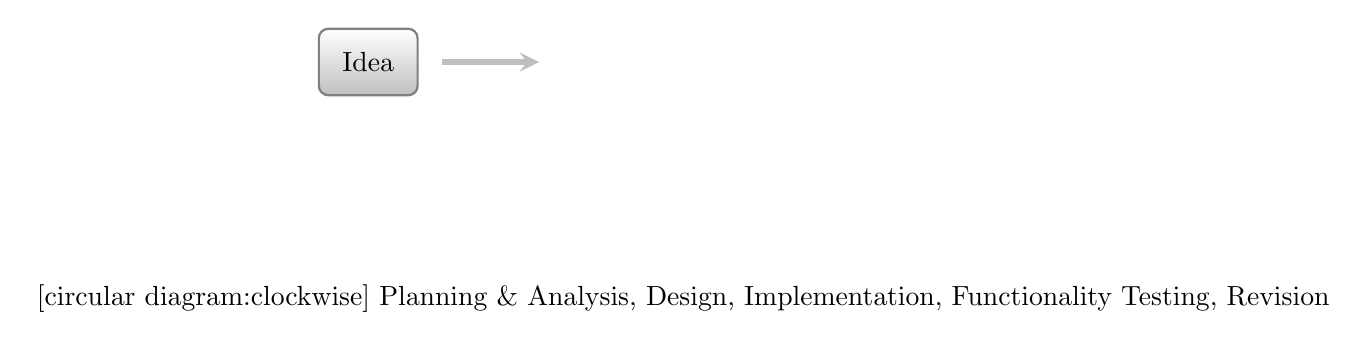
\begin{tikzpicture}[thick]
    \node at (0,0)   {\smartdiagram[circular diagram:clockwise]{
      Planning \& Analysis,
      Design,
      Implementation,
      Functionality Testing,
      Revision}
    };

    \node [rectangle,
           draw=gray,
           rounded corners=0.12 cm,
           inner sep=0.3 cm,
           top color=white,
           bottom color=gray!50]
          (S)  at (-4,3)  {Idea};

    \node (DevI) at (-1.7,3) {};
    \node (StaO) at (-3.2,3) {};

    \path [->,line width=2 pt,gray!50,>=stealth] (StaO) edge (DevI);
  \end{tikzpicture}
  \caption{Scrum development cycle without automated model-based testing.}
  \label{fig:scrumBig}
\end{figure}

The automatic model-generator, described in Section \ref{sec:Technical Implementation}, can aid in the issue, defined above. The tool will allow users to visualize the an intended version of their maritime service instance, before starting implementation, which will enable them to skip the steps 'Implementation', 'Revision', and 'Planning \& Analysis' in a given scrum cycle. In an ideal use case scenario, such as the one, described in %TODO
, as crucial information is given before advancement, a user can, thus, skip large portions of cycles, thereby saving time by not follow dead design ends.

This principle is described by Figure \ref{fig:scrumSmall}, where 'Behavioral Testing' is added to a sub-cycle, only shared with 'Design', thereby creating a much smaller, and considerably faster, sprint.
\newpage
\begin{figure}[h]
  \centering
  \smartdiagramset{arrow line width=2 pt}
  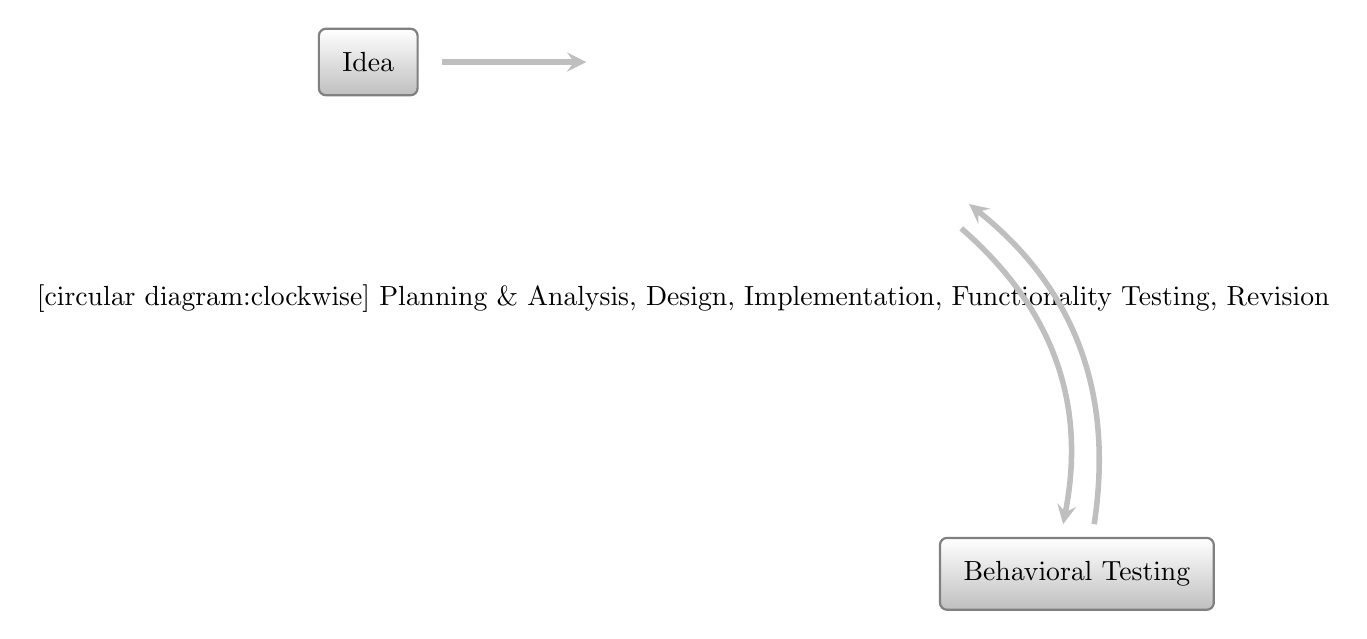
\begin{tikzpicture}[thick]
    \node at (0,0) {\smartdiagram[circular diagram:clockwise]{
      Planning \& Analysis,
      Design,
      Implementation,
      Functionality Testing,
      Revision}
    };

    \node [rectangle,
           draw=gray,
           rounded corners=0.09 cm,
           inner sep=0.3 cm,
           top color=white,
           bottom color=gray!50]
          (S)  at (-4,3)  {Idea};

    \node [rectangle,
           draw=gray,
           rounded corners=0.09 cm,
           inner sep=0.3 cm,
           top color=white,
           bottom color=gray!50]
          (FT)  at (5,-3.5)  {Behavioral Testing};

    \node (DevI) at (-1.1,3) {};
    \node (StaO) at (-3.2,3) {};

    \node (DI)  at (3.5,1.3) {};
    \node (DO)  at (3.4,1) {};

    \node (FTI) at (4.8,-3) {};
    \node (FTO) at (5.2,-3) {};

    \path [->,line width=2 pt,gray!50,>=stealth] (StaO) edge (DevI);
    \path [<-,line width=2 pt,gray!50,>=stealth,bend left] (DI) edge (FTO);
    \path [<-,line width=2 pt,gray!50,>=stealth,bend right] (FTI) edge (DO);
  \end{tikzpicture}
  \caption{Scrum development cycle with automated model-based testing.}
  \label{fig:scrumSmall}
\end{figure}

Manual model generation, in it's basic state, as described in Section \ref{ssec:Expanding Manual Model Functionality}, allows for limitless new functionality, and, as proven by the implementation of the automatic component, said new functionality does not necessarily need to be manual.\\[0.5cm]
In conclusion, both components add relevant functionality to the MCP, and while automatic model generating provides the more present, needed, utility, the manual component provides a broad foundation for development of new ideas.

